\documentclass[11pt]{article}
\usepackage[utf8]{inputenc}

%%%%%%%%%%%%%%%%%%%%%%%%%%%%%%%%%%%%%%%%%%%%%%%%%%%%%%%%%%%%%%%%
% PACKAGES, FORMATTING, LISTING, AND OTHER GRAPHICAL ELEMENTS  %
%%%%%%%%%%%%%%%%%%%%%%%%%%%%%%%%%%%%%%%%%%%%%%%%%%%%%%%%%%%%%%%%

\usepackage{amsmath,amssymb}
\usepackage[T1]{fontenc} % font encoding
\usepackage{graphicx} % for figures
\usepackage{float} % for figures
\usepackage{indentfirst} % indent first paragraph of section
\usepackage{soul,xcolor} % for colors
\usepackage{xkcdcolors} % colors from XKCD color survey
\usepackage{mathtools} % for boxed equations within \align
\usepackage{sectsty} % adjust section headers
\usepackage{fancyhdr} % page headers
\usepackage{titling} % reference title,author,date (in fancyhdr page header)
\usepackage{breqn} % automatically line wrap long Eqs.
\usepackage{pdfpages} % for \includepdf
\usepackage{pdflscape} % landscape 
\usepackage{mdframed} % for framed environment
\usepackage{listings} % for code blocks
\usepackage{inconsolata} % better monospace font
\usepackage{matlab-prettifier} % Better MATLAB listing highlighting
\usepackage[letterpaper, total={6.5in, 9in}]{geometry} % set paper and margin size
\usepackage{empheq} % multiline boxed equations, etc.
\usepackage{hyperref}
\usepackage{dsfont}	% gives you \mathds{} font
% \usepackage{enumerate} % custom enumerate numbering (or lettering in this case)
\usepackage[shortlabels]{enumitem} % more enumerate options
\usepackage{svg} % use inkscape to import svgs
\usepackage{bm} % bold symbols
\usepackage[parfill]{parskip} % replace indentation with paragraph spacing
\usepackage{dsfont} % gives you \mathds{} font

% hyperbolic trig inverse functions
\DeclareMathOperator{\sech}{sech}
\DeclareMathOperator{\csch}{csch}
\DeclareMathOperator{\arcsec}{arcsec}
\DeclareMathOperator{\arccot}{arcCot}
\DeclareMathOperator{\arccsc}{arcCsc}
\DeclareMathOperator{\arccosh}{arcCosh}
\DeclareMathOperator{\arcsinh}{arcsinh}
\DeclareMathOperator{\arctanh}{arctanh}
\DeclareMathOperator{\arcsech}{arcsech}
\DeclareMathOperator{\arccsch}{arcCsch}
\DeclareMathOperator{\arccoth}{arcCoth} 

% add page headers
\pagestyle{fancy}
\fancyhf{}
\fancyhead[LE,LO]{\thetitle}
\fancyhead[RE,RO]{\theauthor}
\fancyfoot[CE,CO]{\thepage}

% adjust section header font size
\sectionfont{\fontsize{20}{15}\selectfont}
\subsectionfont{\fontsize{14}{15}\selectfont}

% vertical table spacing
\renewcommand{\arraystretch}{1.5}

% right-side cases
% \newenvironment{rcases}
%     {\left.\begin{aligned}}
%     {\end{aligned}\right\rbrace}

% Multi-line \fbox
\newcommand\multilineBox[1]{
\noindent
\fbox{
	\parbox{0.97\linewidth}
		{#1}
	}
}

% number just one equation in an un-numbered align* environment
\newcommand\numberthis{\addtocounter{equation}{1}\tag{\theequation}}

%%%%%%%%%%%%%%%%%%%%%%%%%%%%%%%%%%%%%%%%%%%%%%%%%%%%%%%%%%%%%%%%

% set listings font to inconsolata
\DeclareFixedFont{\ttb}{T1}{txtt}{bx}{n}{9} % for bold
\DeclareFixedFont{\ttm}{T1}{txtt}{m}{n}{9}  % for normal

% general listings environment
\lstnewenvironment{code}
{\lstset{
    frame=single,
    % backgroundcolor=\color{xkcdPale},
    basicstyle=\fontfamily{pcr}\selectfont\tiny
    }}
{}

% MATLAB listings environment
\lstnewenvironment{MATLAB}
{\lstset{
    style=Matlab-editor,
    frame=single,
    % backgroundcolor=\color{xkcdPale},
    basicstyle=\fontfamily{pcr}\selectfont\tiny
    }}
{}

% Python style for listings
\newcommand\pythonstyle{\lstset{
    language=Python,
    basicstyle=\ttm,
    morekeywords={self},              % Add keywords here
    keywordstyle=\ttb\color{xkcdGreen},
    morekeywords=[2]{
        array,
        pi,
        zeros,
        max,
        sin,
        cos,
        linspace,
        size,
        plot,
        xlabel,
        title,
        legend,
        show,
        concatenate,
        logspace,
        exp,
        ylabel,
        savefig,
        grid,
        figure,
        axes
    },
    keywordstyle = [2]{\color{xkcdBrightBlue}},
    emph={__init__},                  % Custom highlighting
    emphstyle=\ttb\color{xkcdRed},    % Custom highlighting style
    stringstyle=\color{xkcdGreen},
    backgroundcolor=\color{xkcdPale},
    numberstyle=\color{xkcdGrey},
}}

% Python listings environment
\lstnewenvironment{python}[1][]
{\pythonstyle \lstset{#1}}
{}

% Python listings for external files
\newcommand\pythonexternal[2][]
{{\pythonstyle \lstinputlisting[#1]{#2}}}

% Python listings inline
\newcommand\pythoninline[1]{{\pythonstyle \lstinline!#1!}}


%%%%%%%%%%%%%%%%%%%%%%%%%%%%%%%%%%%%%%%%%%%%%%%%%%%%%%%%%%%%%%%%
% MATHEMATICAL SHORTCUTS                                       %
%%%%%%%%%%%%%%%%%%%%%%%%%%%%%%%%%%%%%%%%%%%%%%%%%%%%%%%%%%%%%%%%

% real and imaginary components
\renewcommand{\Re}{\operatorname{Re}}
\renewcommand{\Im}{\operatorname{Im}}

% Fourier transforms
\newcommand\fourier[1]{\frac{1}{\sqrt{2\pi}} \int_{-\infty}^\infty #1 e^{-i\omega x} \textrm{d}x}
\newcommand\inverseFourier[1]{\frac{1}{\sqrt{2\pi}} \int_{-\infty}^\infty #1 e^{i\omega x} \textrm{d}\omega}

% derivatives
\newcommand{\ppf}[2]{\frac{\partial #1}{\partial #2}}
\newcommand{\pppf}[3]{\frac{\partial^2 #1}{\partial #2 \partial #3}}
\newcommand{\ddf}[2]{\frac{\text{d} #1}{\text{d} #2}}
\newcommand{\DDf}[2]{\frac{\text{D} #1}{\text{D} #2}}

% norms
\newcommand\norm[1]{\lVert#1\rVert}

% statistical operators
\newcommand{\prob}{\operatorname{P}}
\newcommand{\expectation}{\operatorname{E}}
\newcommand{\variance}{\operatorname{Var}}
\newcommand{\stddev}{\operatorname{SD}}

% statistical distributions
\newcommand{\bernoulli}{\operatorname{Bernoulli}}
\newcommand{\binomial}{\operatorname{Binomial}}
\newcommand{\poisson}{\operatorname{Poisson}}
\newcommand{\normal}{\operatorname{Normal}}

%%%%%%%%%%%%%%%%%%%%%%%%%%%%%%%%%%%%%%%%%%%%%%%%%%%%%%%%%%%%%%%%
% COMMONLY USED COPYPASTAS
%%%%%%%%%%%%%%%%%%%%%%%%%%%%%%%%%%%%%%%%%%%%%%%%%%%%%%%%%%%%%%%%

% CODE BLOCK

% \begin{MATLAB}[caption={MATLAB script},label={code:p1}]
% for i = 1:n
%     disp('string')
% end
% \end{MATLAB}
% Code block \ref{code:p1}



% MULTIPLE EQUATIONS BOXED

% \begin{empheq}[box=\fbox]{align}
% \end{empheq}



% ENUMERTATE WITH a) instead of 1.

% \begin{enumerate}[label=\alph*)]
% \end{enumerate}
% 'Problem' sections
% \renewcommand{\thesection}{Part \arabic{section}}
\renewcommand{\thesubsection}{\arabic{section}.\alph{subsection}}
% \renewcommand{\thesubsection}{\arabic{subsection}}

\title{ENGR 510 Statistics Homework}
\author{Anthony Su}
\date{November 22, 2024}

\begin{document}
\thispagestyle{plain}
\maketitle


%%%%%%%%%%%%%%%%%%%%%%%%%%%%%%%%%%%%%%%%%%%%%%%%%%%%%%%%%%%%%%%%%%%%%%%%%%%%%%%%
% 1. Intro to Probability
%%%%%%%%%%%%%%%%%%%%%%%%%%%%%%%%%%%%%%%%%%%%%%%%%%%%%%%%%%%%%%%%%%%%%%%%%%%%%%%%
\section{Intro to Probability}

\subsection{}  % a -------------------------------------------------------------
Using a brute force enumeration technique, the result is
\begin{align*}
    \Aboxed{
        \prob(S=10) &= 0.125
    }
\end{align*}

\subsection{}  % b -------------------------------------------------------------
Due to the central limit theorem, this system can be modeled as normally
distributed. For a single roll with $\omega = \{1, 2, 3, 4, 5, 6\}$,
\begin{align*}
    \expectation (X_i) &= \frac{1}{6} \sum_{i=1}^{6} \omega_i \\
    \expectation (X_i) &= 3.5
\end{align*}
and the variance is
\begin{align*}
    \variance (X_i) &= \frac{1}{6} \sum_{i=1}^{6} \left( \omega_i - 3.5 \right)^2 \\
    \variance (X_i) &= \frac{35}{12}
\end{align*}
Thus, the mean and variance for the average of 100 rolls can be modeled by $\mathcal{N}\left(3.5, \sqrt{\frac{35}{12}}\right)$.
For the sum of 100 rolls, this becomes $\mathcal{N}\left(350, \sqrt{100 \cdot \frac{35}{12}}\right)$.

Integrating the PDF of this distribution from $299.5$ to $300.5$ (one unit around $300$)
yields a probability of approximately $0.03\%$ to roll a sum of exactly $300$.
Integrating the PDF of this distribution from $-\infty$ to $299.5$ yields a
probability of approximately $0.16\%$ to roll a sum of $\leq300$.

\begin{align*}
    \Aboxed{
        \prob(S=300) &\approx 0.03\%
    } \\
    \Aboxed{
        \prob(S<300) &\approx 0.16\%
    }
\end{align*}

\subsection{}  % c -------------------------------------------------------------
There are $6^5$ ways to roll 5 dice.
There are $5^5$ ways to roll no ones for each of of the 5 dice.
There are $5^4$ ways to roll 1 one with any given die.
Thus, there are $5 \times 5^4$ ways to roll 1 one out of 5 rolls.

The probability of rolling 2 or more ones is
\begin{equation*}
    \prob(\text{snake eyes}) = 1-\prob(\text{0 ones})-\prob(\text{1 one})
\end{equation*}
Substituting in values,
\begin{align*}
    \prob(\text{snake eyes}) &= 1-\frac{5^5}{6^5}-\frac{5 \cdot 5^4}{6^5} \\
    \prob(\text{snake eyes}) &= 1-2\cdot\left(\frac{5}{6}\right)^5 \\
    \Aboxed{
        \prob(\text{snake eyes}) &\approx 19.62\%
    }
\end{align*}

\subsection{}  % d -------------------------------------------------------------

There are ${6 \choose 2}=15$ ways to place the two numbers within the license
plate. For each placement of letters and numbers, there are $26^4 * 10^2$ ways
to assign letters and numbers. Thus, the total number of possible license plates
is
\begin{align*}
    |\Omega| &= {6 \choose 2} \cdot 26^4 \cdot 10^2 \\
    \Aboxed{
        |\Omega| &= 685,464,000
    }
\end{align*}

\subsection{}  % e -------------------------------------------------------------
The number of license plates with no repeated characters is
\begin{align*}
    |\Omega^\prime| = {6 \choose 2}\cdot \frac{26!}{(26-4)!} \cdot \frac{10!}{(10-2)!}
\end{align*}
Thus, the number of license plates with repeated characters is
\begin{align*}
    |\Omega| - |\Omega^\prime| &= {6 \choose 2}\left(
        26^4 \cdot 10^2 - \frac{26!}{(26-4)!} \cdot \frac{10!}{(10-2)!}
    \right) \\
    \Aboxed{
        |\Omega|-|\Omega^\prime| &= 201,084,000
    }
\end{align*}

\subsection{}  % f -------------------------------------------------------------
There are four ways for a license plate to have the word "CAT":
\begin{table}[H]
    \centering{}
    \caption{Locations of "CAT" on license plates}
    \label{1ftab1}
    \begin{tabular}{c}
        \hline\hline
        C A T _ _ _ \\
        _ C A T _ _ \\
        _ _ C A T _ \\
        _ _ _ C A T \\
        \hline\hline
    \end{tabular}
\end{table}
For each of those ways, the remaining letter can be placed in one of the three
remaining slots; there are ${3 \choose 1}=3$ ways to do this. For each of those
ways, the number of outcomes for the remaining one letter and two numbers is
$26 * 10 * 10 = 2600$. The total number of ways for the license plate to have
the word "CAT" is
\begin{align*}
    |\Omega'| &= 4 \cdot 3 \cdot 2600
\end{align*}
Thus, the number of license plates without the word "CAT" is
\begin{align*}
    |\Omega|-|\Omega'| &= {6 \choose 2} \cdot 26^4 \cdot 10^2 - 4 \cdot 3 \cdot 2600 \\
    \Aboxed{
        |\Omega|-|\Omega'| &= 685,432,800
    }
\end{align*}

%%%%%%%%%%%%%%%%%%%%%%%%%%%%%%%%%%%%%%%%%%%%%%%%%%%%%%%%%%%%%%%%%%%%%%%%%%%%%%%%
% 2. Birthday Problem
%%%%%%%%%%%%%%%%%%%%%%%%%%%%%%%%%%%%%%%%%%%%%%%%%%%%%%%%%%%%%%%%%%%%%%%%%%%%%%%%
\section{Birthday Problem}

\subsection{}  % a -------------------------------------------------------------
\begin{equation*}
    P(\geq2 \text{ share}) = \prod_{k=0}^{N-1} \frac{365-k}{365}
\end{equation*}
\begin{mdframed}
    There must be at least 32 people for the chance of a shared birthday to be
    over 75\%.
\end{mdframed}

\subsection{}  % b -------------------------------------------------------------
There are many ways for people to share birthdays without forming a triplet.
This precludes the traditional birthday problem approach of further subtracting
the probabilities of all outcomes with exclusively birthday pairs. Thus, in lieu of an
exact/analytical solution,
\begin{mdframed}
    I would approach this problem with a Monte Carlo simulation.
\end{mdframed}

%%%%%%%%%%%%%%%%%%%%%%%%%%%%%%%%%%%%%%%%%%%%%%%%%%%%%%%%%%%%%%%%%%%%%%%%%%%%%%%%
% 3. Monte Carlo
%%%%%%%%%%%%%%%%%%%%%%%%%%%%%%%%%%%%%%%%%%%%%%%%%%%%%%%%%%%%%%%%%%%%%%%%%%%%%%%%
\section{Monte Carlo}

\subsection{}  % a -------------------------------------------------------------
The chance of landing in the largest sphere that fits inside the cube is equal
to the ratio of the volumes of the sphere and the cube:
\begin{align*}
    P(\text{inside}) &= \frac{(1/6) \pi L^3}{L^3} \\
    \Aboxed{
        P(\text{inside}) &= \frac{\pi}{6}
    }
\end{align*}

\subsection{}  % b -------------------------------------------------------------
\begin{python}[caption={},label={3blst1}]
def sample_hypercube(n):
    x = np.random.random_sample(size=n) * 2 - 1  # rescale to [-1, 1]
    r = np.linalg.norm(x)
    if r < 1:
        return True
    elif r > 1:
        return False
\end{python}

\subsection{}  % c -------------------------------------------------------------
\begin{python}[caption={},label={3clist1}]
N_samples = 10000
N_in = 0
for i in range(N_samples):
    if sample_hypercube(3):
        N_in += 1
print(f'Number of points within sphere for 3D cubic domain: {N_in}')
\end{python}
\begin{mdframed}
Out of 10000 samples, 5118 were within the sphere, which is 51.18\%.
\end{mdframed}

\subsection{}  % d -------------------------------------------------------------
\begin{figure}[H]
    \centering
    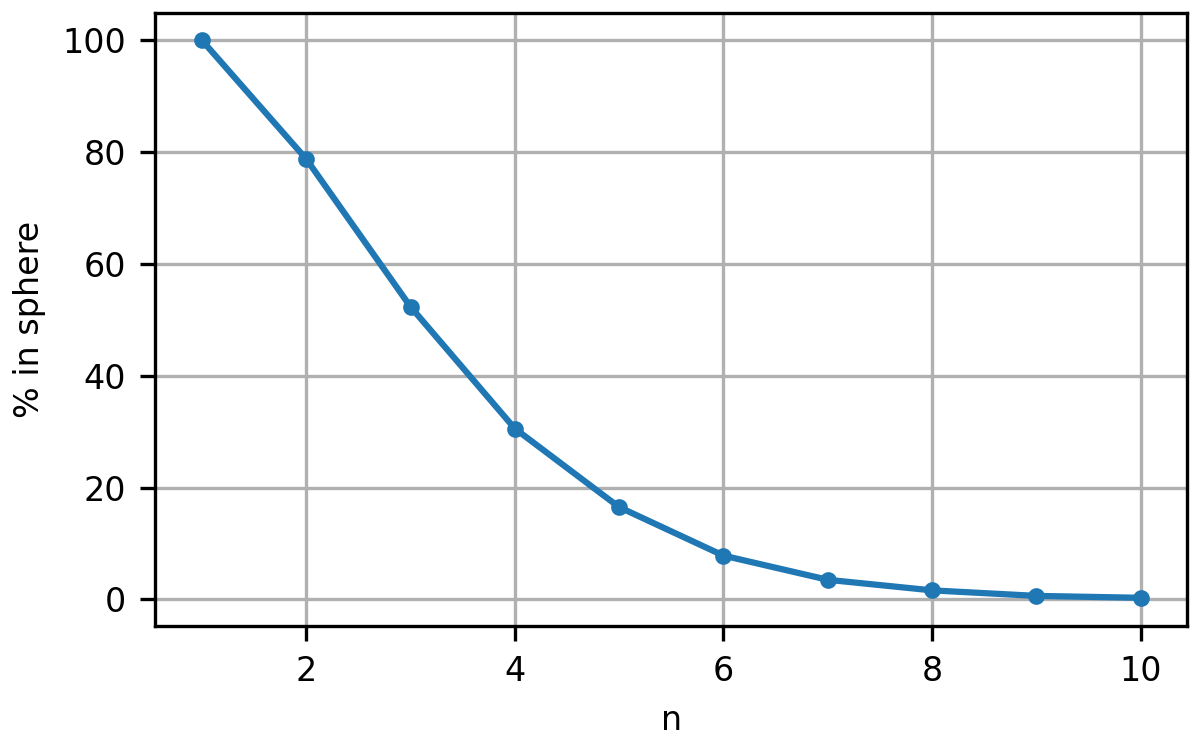
\includegraphics[width=4in]{3dfig1.png}
    \caption{Chance of being in the unit sphere for $n$ dimensions}
    \label{3dfig1}
\end{figure}
\begin{mdframed}
    As $n$ increases, the probability of sampling a point within a unit radius of
    the origin rapidly approaches zero.
\end{mdframed}

\subsection{}  % e -------------------------------------------------------------

Each value $X_i$ in Figure \ref{3dfig1} is a realization of a binomially distributed
random variable $X$:
\begin{align*}
    X \sim \binomial(N, p)
\end{align*}
From the law of large numbers, we know $\mu = p = \bar{X}_i$.
% The variance of a binomially distributed variable is
% \begin{align*}
%     \variance(X) &= \expectation\left(X^2\right) - \expectation(X)^2
% \end{align*}
% Since Bernoulli outcomes are binary, $\expectation\left(X^2\right) = \expectation\left(X\right)$.
% Furthermore, $\expectation(X) = p = \bar{X}_i$. Thus,
% \begin{align*}
%     \variance(X) &= p - p^2 \\
%     \variance(X) &= p (1-p) \\
%     \variance(X) &= \bar{X}_i (1-\bar{X}_i)
% \end{align*}
% Thus, variances for the values shown in Figures \ref{3dfig1} are computed and shown
% in Table \ref{3etab1}. The 95\% confidence intervals are then computing using the
% CDF of a normal approximation for the binomially distributed $X$ given by
% \begin{align*}
%     X \sim \mathcal{N}(\bar{X}, \variance(X))
% \end{align*}
The variance can be computed for a given $n$ by
\begin{align*}
    \hat{\sigma}^2 &= \frac{1}{n} \sum_{i=1}^{n} \left(X_i - \bar{X}\right)^2
\end{align*}
This variance can then be used in the normal approximation to compute 95\%
confidence intervals.

\begin{mdframed}
\begin{table}[H]
    \centering
    \caption{95\% confidence intervals for various $n$}
    \begin{tabular}{cccc}
        \hline\hline
        $n$ & $\sigma^2$ & upper bound (\%) & lower bound (\%) \\
        \hline
        1  & 0.0      & 100   & 100   \\
        2  & 1.64e-05 & 78.62 & 80.20 \\
        3  & 2.49e-05 & 51.73 & 53.69 \\
        4  & 2.16e-05 & 30.63 & 32.45 \\
        5  & 1.41e-05 & 16.32 & 17.80 \\
        6  & 7.35e-06 & 7.46  & 8.52  \\
        7  & 3.69e-06 & 3.46  & 4.22  \\
        8  & 1.55e-06 & 1.33  & 1.81  \\
        9  & 6.66e-07 & 0.51  & 0.83  \\
        10 & 2.39e-07 & 0.14  & 0.34  \\
        \hline\hline
    \end{tabular}
    \label{3etab1}
\end{table}
\end{mdframed}

Note that $\sigma^2$ is approximated as $\hat{\sigma}^2/N$.

Note that at higher values of $n$, the normal distribution becomes a poorer approximation
to the binomial distribution since $p \ll 1$. However, with the large sample size of
$N=10,000$, this issue is somewhat mitigated.

%%%%%%%%%%%%%%%%%%%%%%%%%%%%%%%%%%%%%%%%%%%%%%%%%%%%%%%%%%%%%%%%%%%%%%%%%%%%%%%%
% 4. Central Limit Theorem
%%%%%%%%%%%%%%%%%%%%%%%%%%%%%%%%%%%%%%%%%%%%%%%%%%%%%%%%%%%%%%%%%%%%%%%%%%%%%%%%
\section{Central Limit Theorem}

\subsection{}  % a -------------------------------------------------------------
\begin{figure}[H]
    \centering
    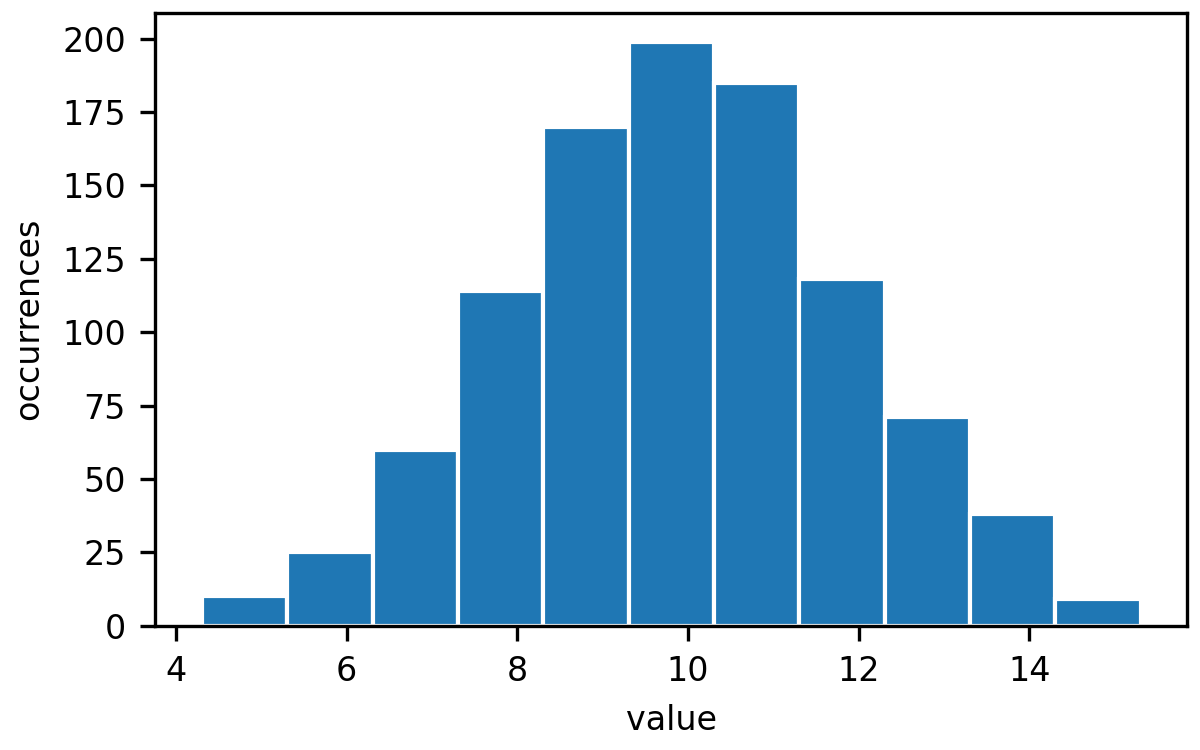
\includegraphics[width=4in]{4afig1.png}
    \caption{Example normally-distributed sequence with $n=1000$}
    \label{4afig1}
\end{figure}
\begin{figure}[H]
    \centering
    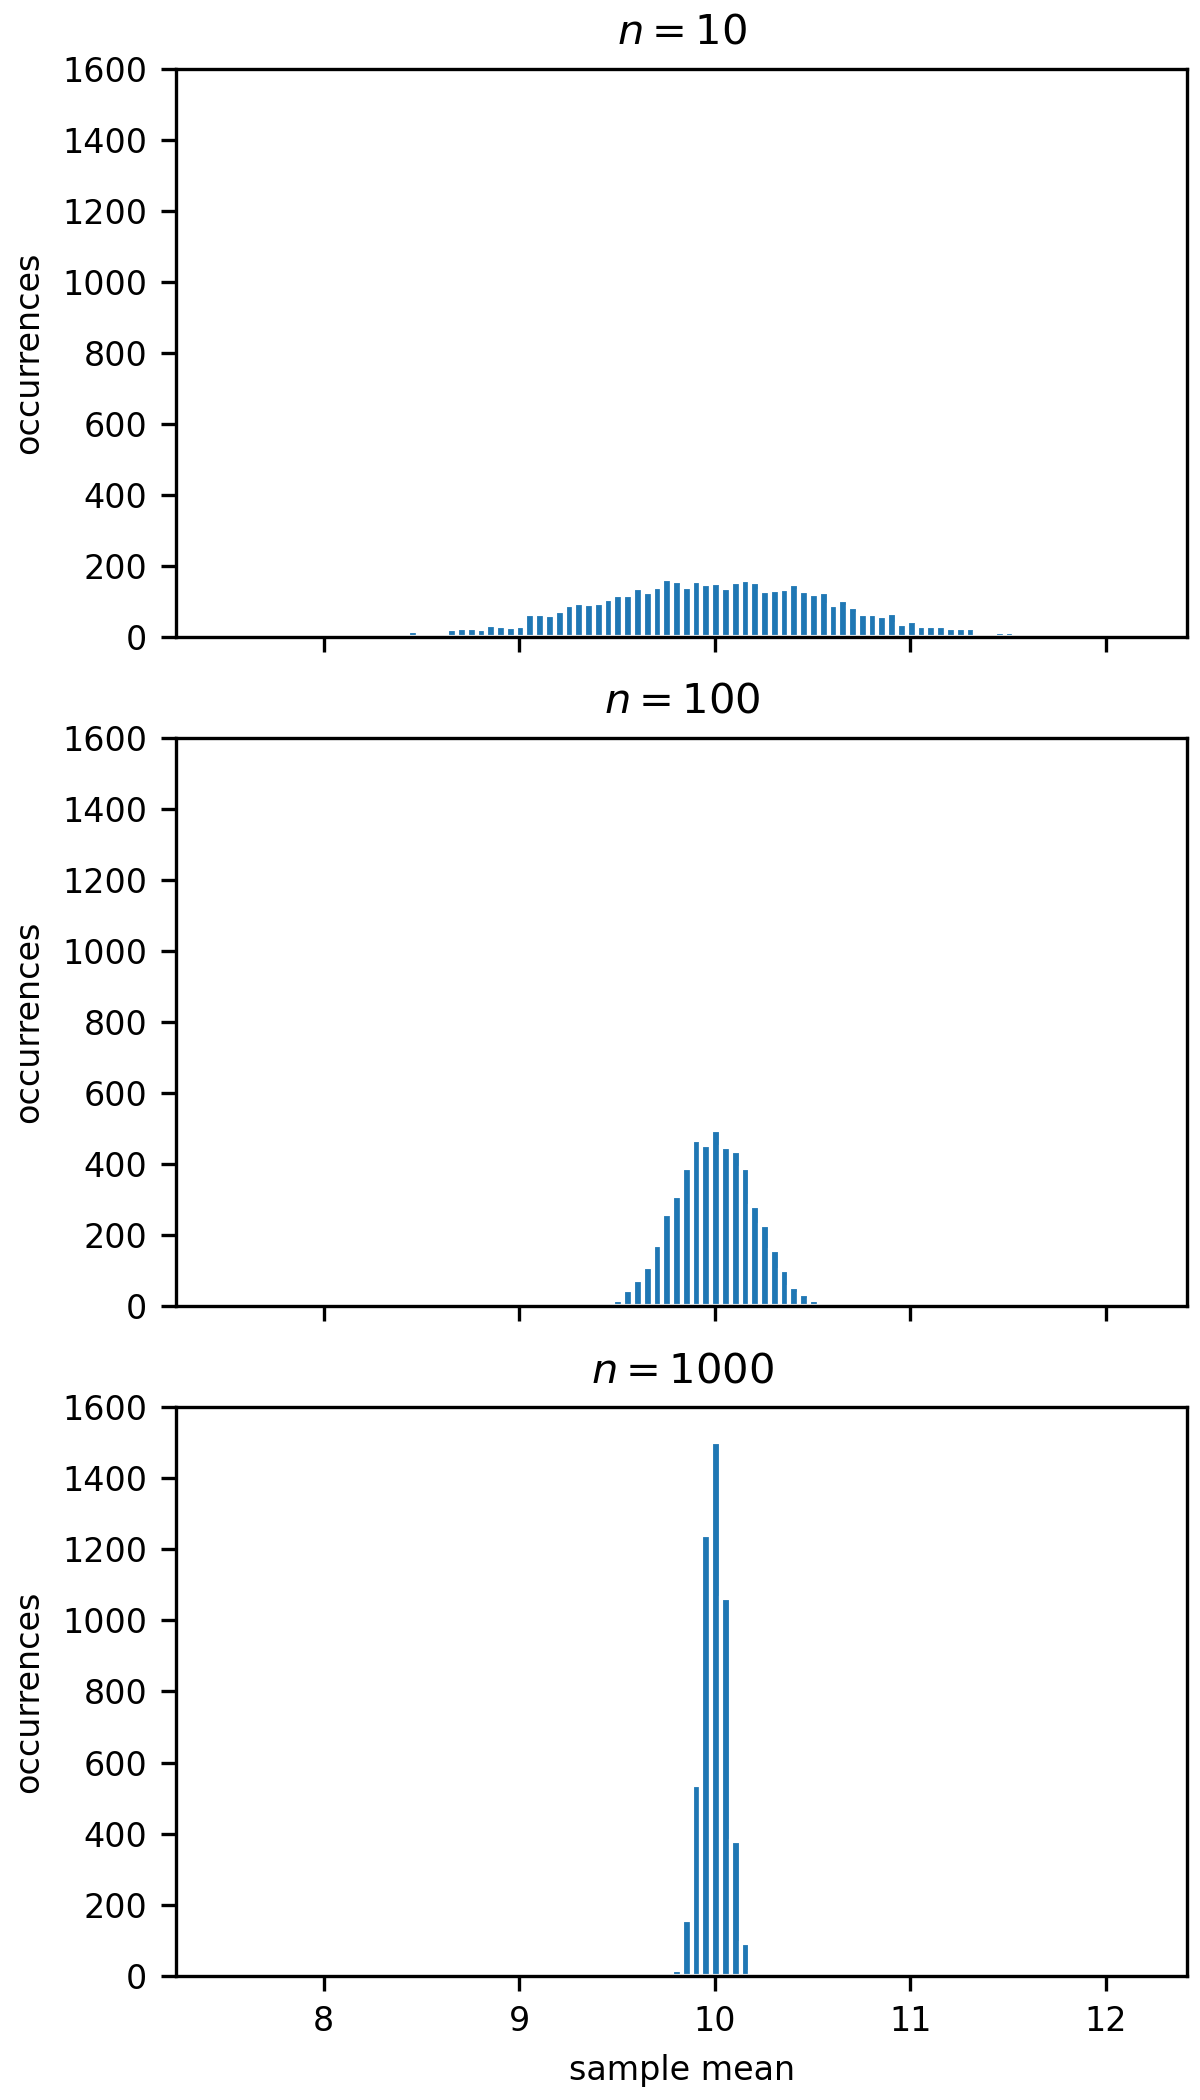
\includegraphics[width=4in]{4afig2.png}
    \caption{Sample means for normally-distributed sequences with $n=\{10, 100, 1000\}$}
    \label{4afig2}
\end{figure}

\subsection{}  % b -------------------------------------------------------------
\begin{figure}[H]
    \centering
    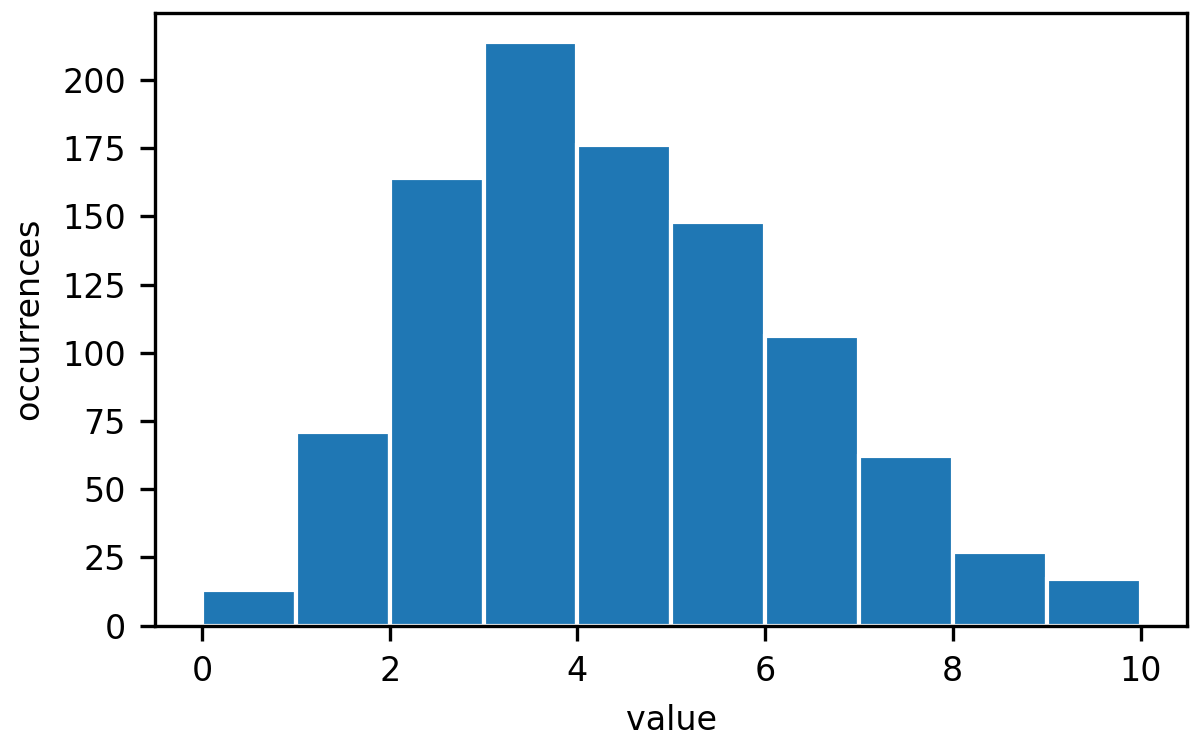
\includegraphics[width=4in]{4bfig1.png}
    \caption{Example Poisson-distributed sequence with $n=1000$}
    \label{4bfig1}
\end{figure}
\begin{figure}[H]
    \centering
    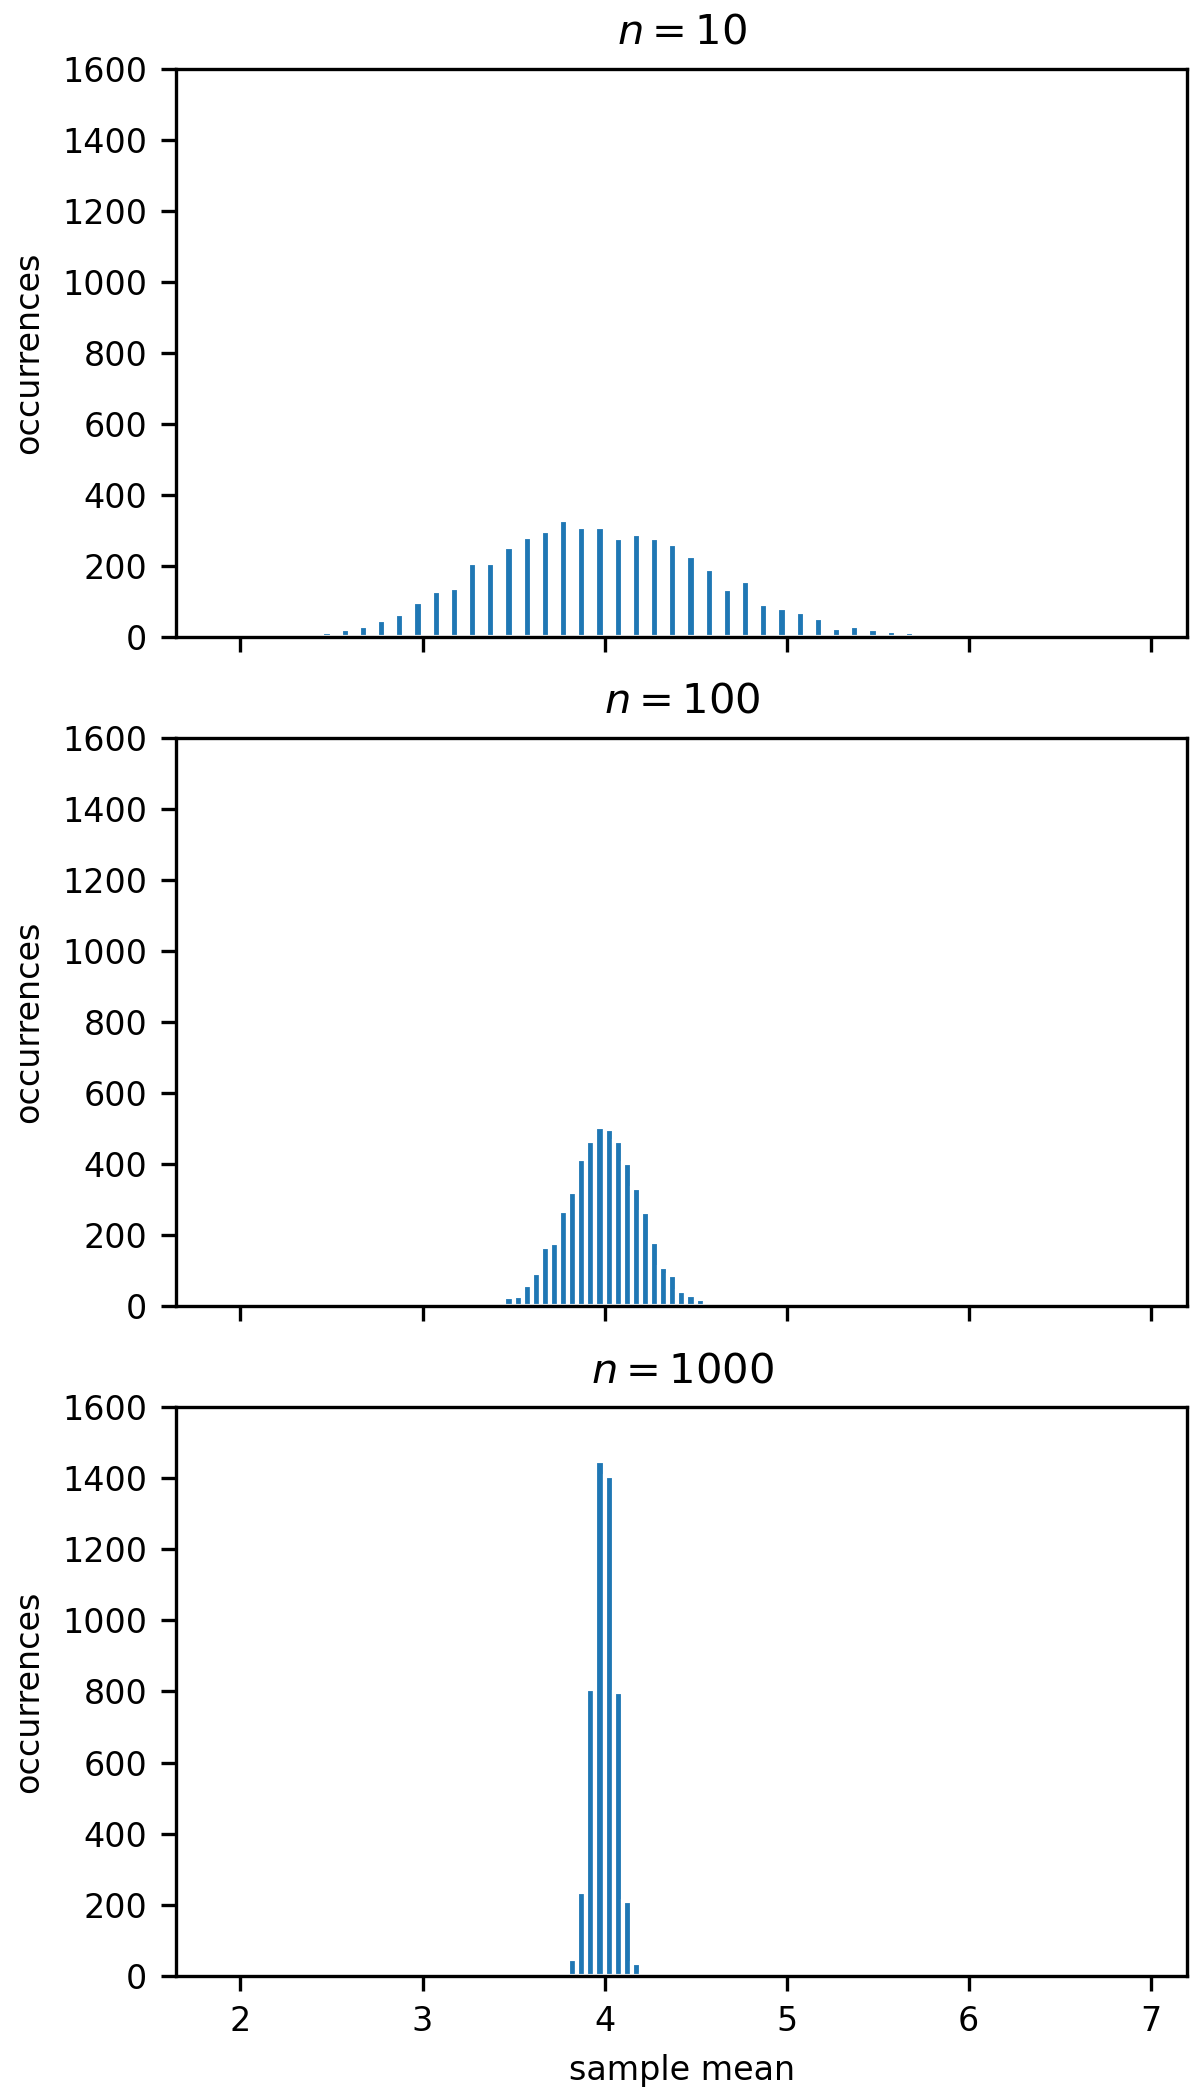
\includegraphics[width=4in]{4bfig2.png}
    \caption{Sample means for Poisson-distributed sequences with $n=\{10, 100, 1000\}$}
    \label{4bfig2}
\end{figure}

\subsection{}  % c -------------------------------------------------------------
\begin{figure}[H]
    \centering
    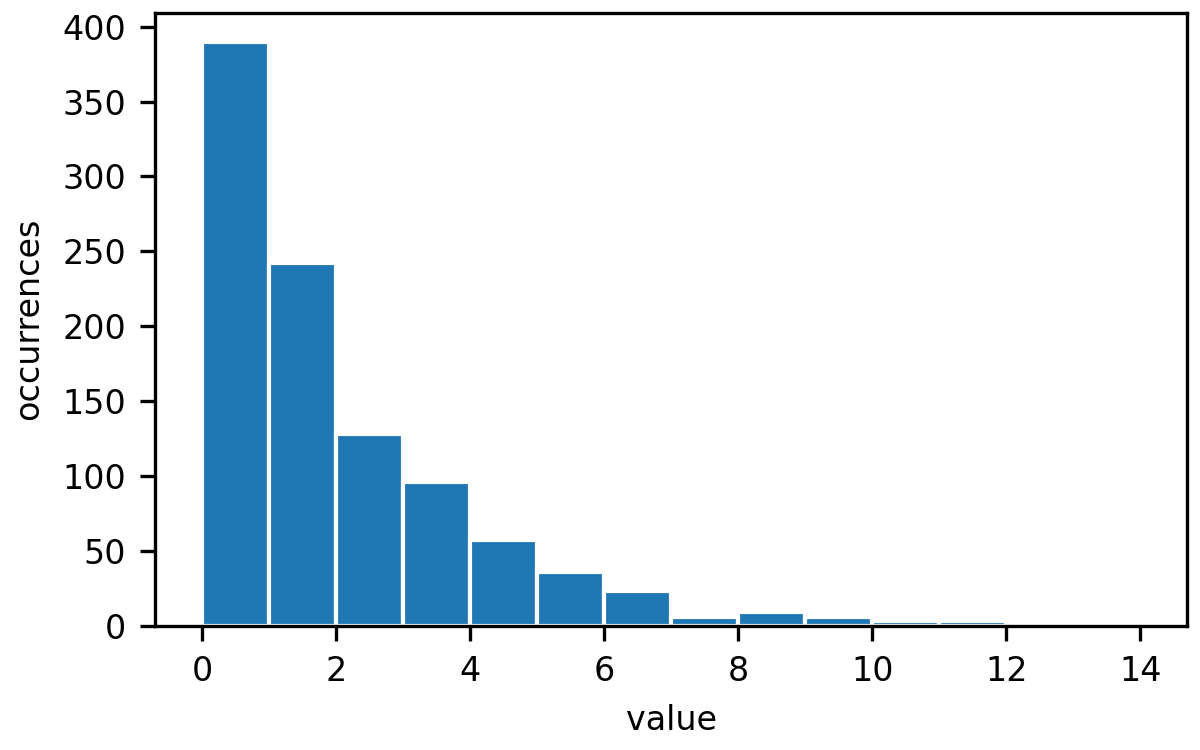
\includegraphics[width=4in]{4cfig1.png}
    \caption{Example Gamma-distributed sequence with $n=1000$}
    \label{4cfig1}
\end{figure}
\begin{figure}[H]
    \centering
    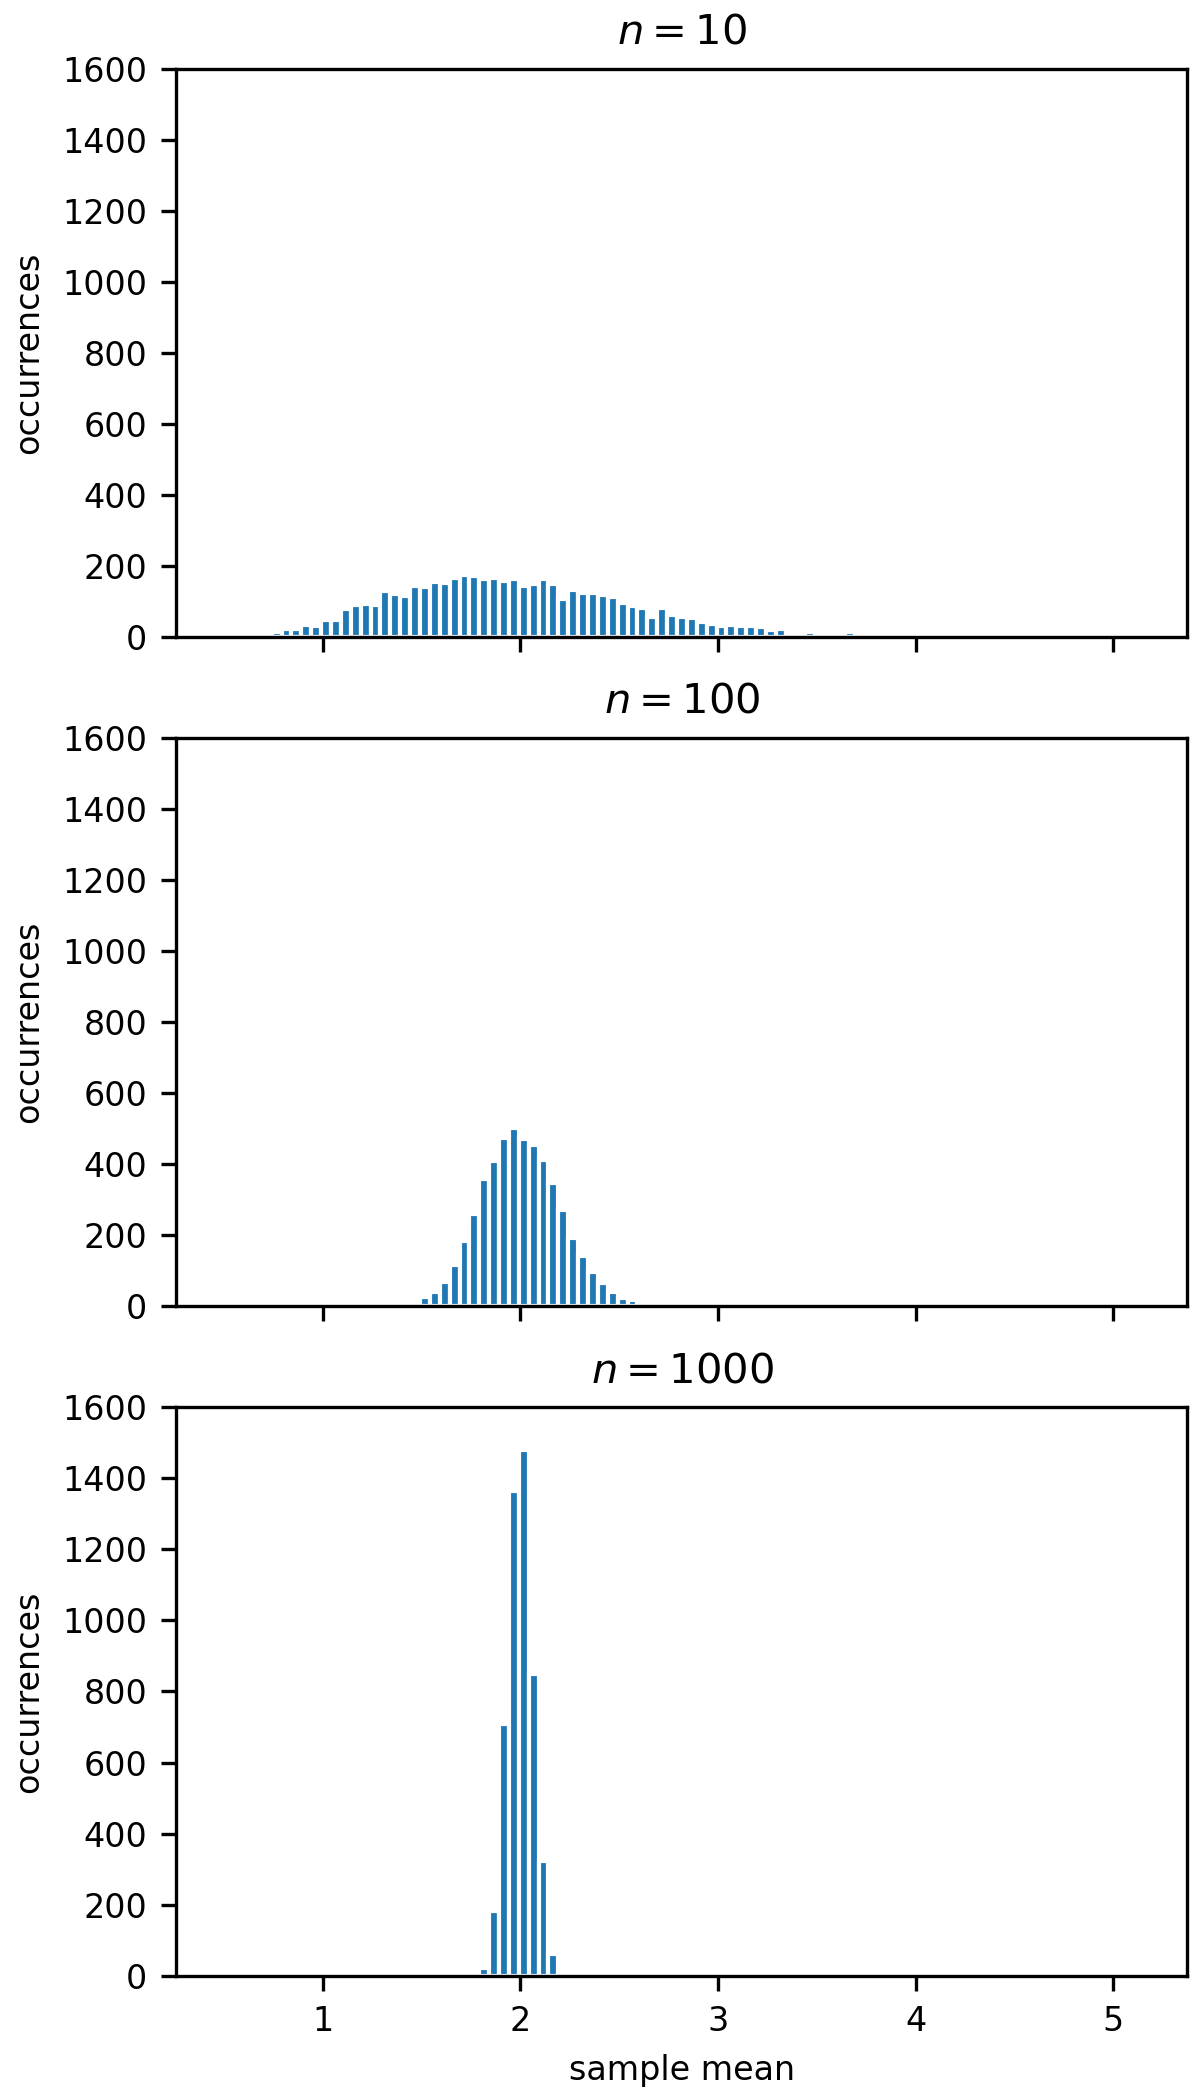
\includegraphics[width=4in]{4cfig2.png}
    \caption{Sample means for Gamma-distributed sequences with $n=\{10, 100, 1000\}$}
    \label{4cfig2}
\end{figure}

%%%%%%%%%%%%%%%%%%%%%%%%%%%%%%%%%%%%%%%%%%%%%%%%%%%%%%%%%%%%%%%%%%%%%%%%%%%%%%%%
% 5. Conditional Probability
%%%%%%%%%%%%%%%%%%%%%%%%%%%%%%%%%%%%%%%%%%%%%%%%%%%%%%%%%%%%%%%%%%%%%%%%%%%%%%%%
\section{Conditional Probability}

\begin{align*}
    P(\text{defect}) &= 0.05 & P(\text{no defect}) &= 0.95 \\
    P(\text{positive}|\text{defect}) &= 0.9 & P(\text{negative}|\text{defect}) &= 0.1 \\
    P(\text{positive}|\text{no defect}) &= 0.1 & P(\text{negative}|\text{no defect}) &= 0.9
\end{align*}

\subsection{}  % a -------------------------------------------------------------
\begin{align*}
    P(\text{defect}|\text{positive}) &= \frac{
        P(\text{positive}|\text{defect}) \cdot P(\text{defect})
        }{
        P(\text{positive}|\text{defect}) \cdot P(\text{defect})
        + P(\text{positive}|\text{no defect}) \cdot P(\text{no defect})
        } \\
    P(\text{defect}|\text{positive}) &= \frac{
        0.9 \cdot 0.05
        }{
        0.9 \cdot 0.05 + 0.1 \cdot 0.95
        } \\
    \Aboxed{
        P(\text{defect}|\text{positive}) &= 32.14\%
    }   
\end{align*}

\subsection{}  % b -------------------------------------------------------------
% \begin{align*}
%     P(\text{no defect}|\text{positive}) &= \frac{
%         P(\text{positive}|\text{no defect}) \cdot P(\text{no defect})
%         }{
%         P(\text{positive}|\text{no defect}) \cdot P(\text{no defect})
%         + P(\text{positive}|\text{defect}) \cdot P(\text{defect})
%         } \\
%     P(\text{no defect}|\text{positive}) &= \frac{
%         0.1 \cdot 0.95
%         }{
%             0.1 \cdot 0.95 + 0.9 \cdot 0.05
%         } \\
%     P(\text{defect}|\text{positive}) &= 67.86\%
% \end{align*}
\begin{align*}
    P(\text{no defect}|\text{positive}) &= 1 - P(\text{defect}|\text{positive}) \\
    \Aboxed{
        P(\text{no defect}|\text{positive}) &= 67.86\%
    }
\end{align*}

\subsection{}  % c -------------------------------------------------------------
As given,
\begin{align*}
    \Aboxed{
        P(\text{positive}|\text{no defect}) &= 0.1
    }
\end{align*}

%%%%%%%%%%%%%%%%%%%%%%%%%%%%%%%%%%%%%%%%%%%%%%%%%%%%%%%%%%%%%%%%%%%%%%%%%%%%%%%%
% 6. Statistical Data Analysis
%%%%%%%%%%%%%%%%%%%%%%%%%%%%%%%%%%%%%%%%%%%%%%%%%%%%%%%%%%%%%%%%%%%%%%%%%%%%%%%%
\section{Statistical Data Analysis}

\subsection{}  % a -------------------------------------------------------------

\begin{figure}[H]
    \centering
    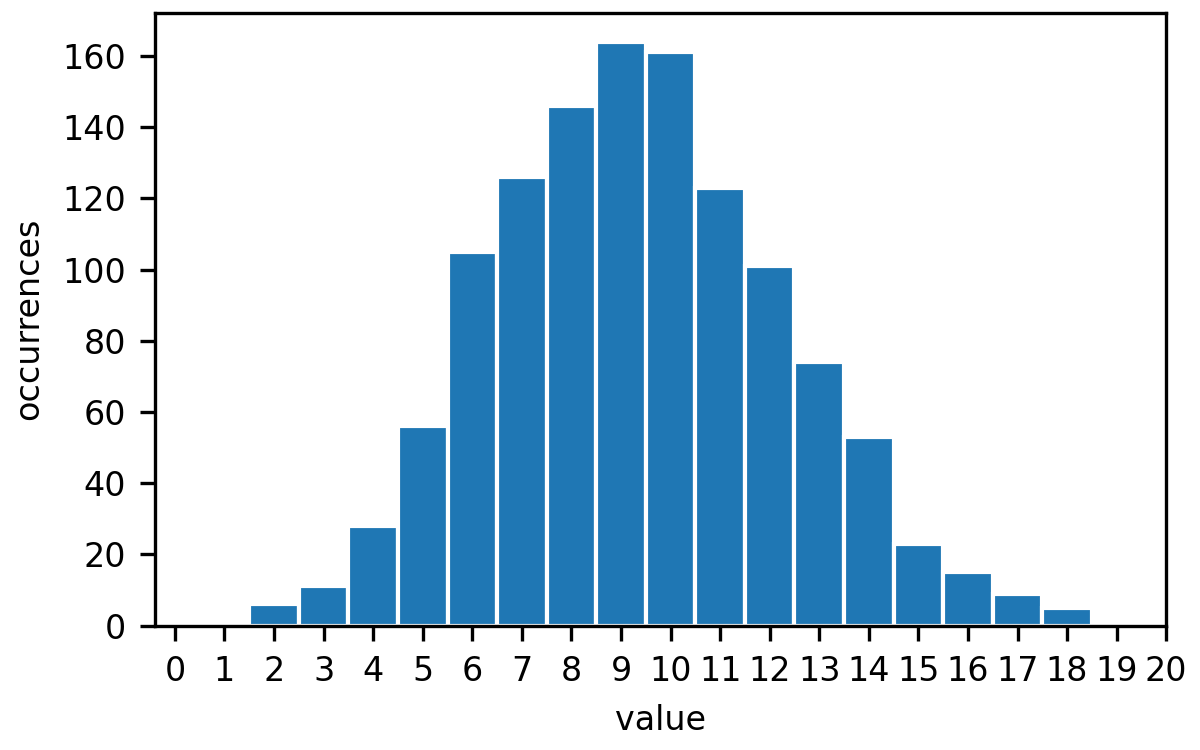
\includegraphics[width=4in]{6afig1.png}
    \caption{Problem 6 data}
    \label{6afig1}
\end{figure}

\subsection{}  % b -------------------------------------------------------------
\begin{mdframed}
    The sample mean is $\bar{X}=9.36$ and the sample variance is $\hat{\sigma}^2=8.62$.
\end{mdframed}

\subsection{}  % c -------------------------------------------------------------
\begin{figure}[H]
    \centering
    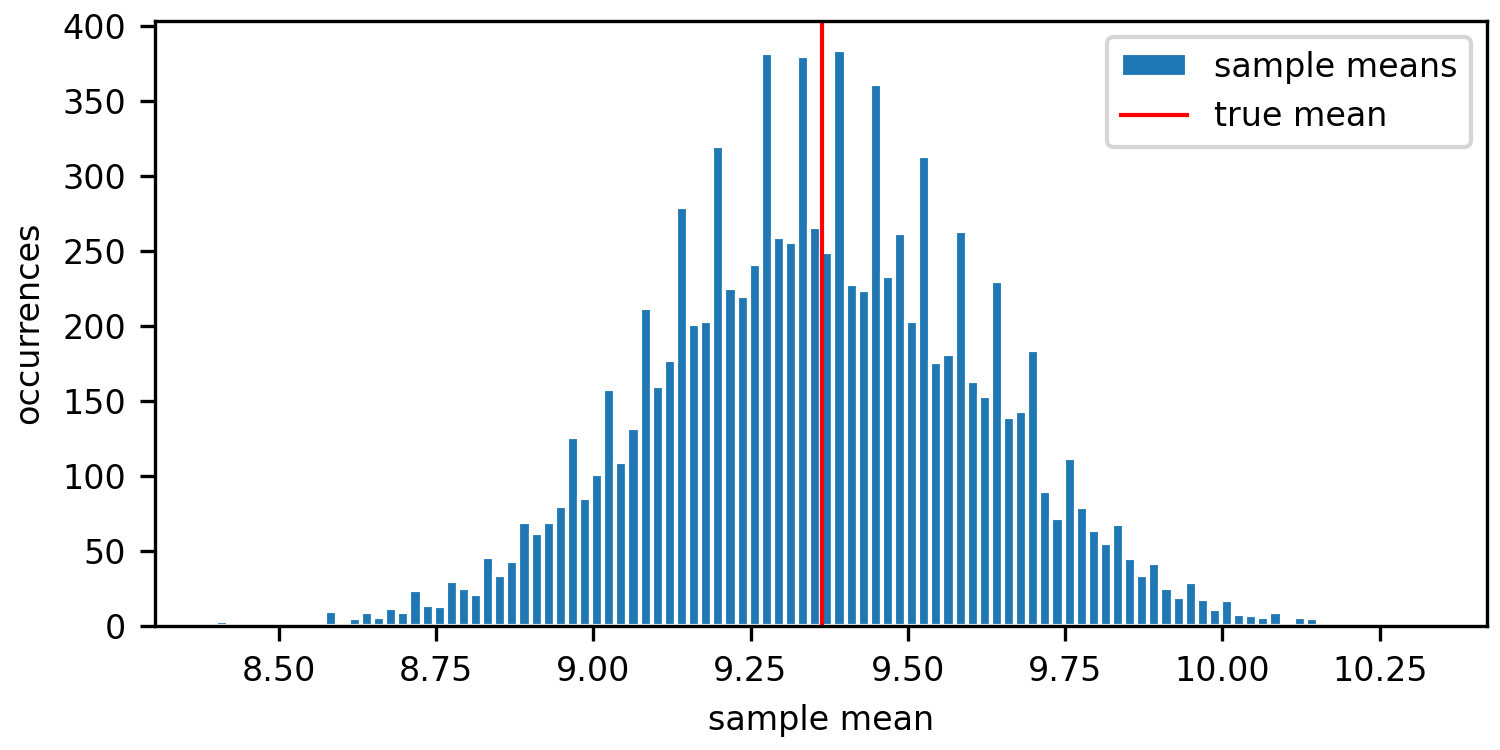
\includegraphics[width=5in]{6cfig1.png}
    \caption{10\% subset sample means}
    \label{6cfig1}
\end{figure}
\begin{figure}[H]
    \centering
    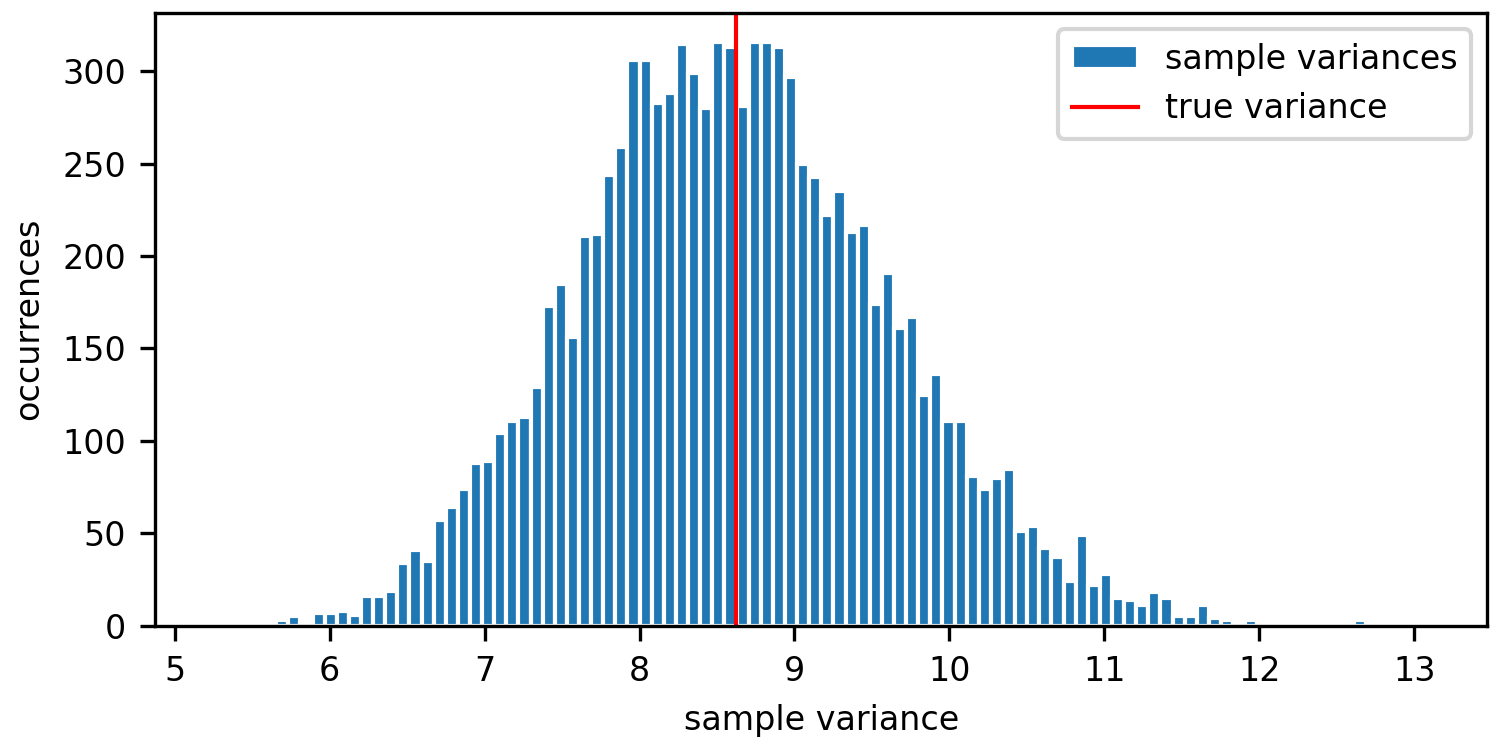
\includegraphics[width=5in]{6cfig2.png}
    \caption{10\% subset sample variances}
    \label{6cfig2}
\end{figure}
\begin{mdframed}
    This is consistent with the expectation from the central limit theorem
    because the sample means and variances are normally distributed about the
    true mean and variance.
\end{mdframed}

\subsection{}  % d -------------------------------------------------------------
\subsubsection{Method of Moments}
Assume a sample $X_i$ is distributed as $X_i\sim\poisson(\lambda)$.

$\lambda$ is defined as
\begin{align*}
    \lambda &= \mu_1 \\
    \lambda &= \expectation (X_i) \\
\end{align*}
Due to the law of large numbers, this is
\begin{align*}
    \lambda &= \bar{X}_i \\
    \lambda &= 9.36
\end{align*}
\begin{mdframed}
    Using the method of moments, $X_i \sim \poisson(9.36)$
\end{mdframed}

\subsubsection{MLE}
Assume a sample $X_i$ is distributed as $X_i\sim\poisson(\lambda)$.

The distribution function is
\begin{align*}
    f(x_1, \dots, x_n | \lambda) &= \prod_{i=1}^{n} \frac{\lambda^{x_i} e^{-\lambda}}{x_{i}!}
\end{align*}
The log-likelihood function is
\begin{align*}
    l(X_1, \dots, X_n | \lambda) &= \log\left(f(X_1, \dots, X_n | \lambda)\right) \\
    l(X_1, \dots, X_n | \lambda) &= \log\left(\prod_{i=1}^{n} \frac{\lambda^{X_i} e^{-\lambda}}{X_i!}\right) \\
    l(X_1, \dots, X_n | \lambda) &= \sum_{i=1}^{n} \left[ X_i \log(\lambda) - \lambda - \log(X_i!)\right]
\end{align*}
Taking the derivative,
\begin{align*}
    \ppf{l}{\lambda}(X_1, \dots, X_n | \lambda) &= \sum_{i=1}^{n} \left[ \frac{1}{\lambda} X_i - 1 \right] \\
    \ppf{l}{\lambda}(X_1, \dots, X_n | \lambda) &= \frac{n}{\lambda} \bar{X}_i - n
\end{align*}
Equating the derviative to zero,
\begin{align*}
    \ppf{l}{\lambda}(X_1, \dots, X_n | \lambda) &= 0 \\
    \frac{n}{\lambda} \bar{X}_i - n &= 0 \\
    \bar{X}_i &= \lambda
\end{align*}
Thus, $\lambda = \bar{X}_i$ is a critical point of the distribution log-likelihood function.

Taking the second derivative,
\begin{align*}
    \pppf{l}{\lambda^2}(X_1, \dots, X_n | \lambda) &= \frac{n}{\lambda} \bar{X}_i - n \\
    \pppf{l}{\lambda^2}(X_1, \dots, X_n | \lambda) &= - \frac{n}{\lambda^2} \bar{X}_i
\end{align*}
Evaluating the second derivative at the critical point,
\begin{align*}
    \pppf{l}{\lambda^2}(X_1, \dots, X_n | \lambda=\bar{X}_i) &= - \frac{n}{\bar{X}_i^2} \bar{X}_i \\
    \pppf{l}{\lambda^2}(X_1, \dots, X_n | \lambda=\bar{X}_i) &= - \frac{n}{\bar{X}_i}
\end{align*}
Since $\bar{X}_i > 0$, this second derivative is negative. Since $\lambda = \bar{X}_i$
is a critical point of $l(X_1, \dots, X_n | \lambda)$ with negative second derivative,
it is a maximum.
\begin{mdframed}
    Thus, $\poisson(9.36)$ is the maximum-likelihood estimate of $X_i$.
\end{mdframed}

\subsection{}  % e -------------------------------------------------------------
% Assume that $X_i \sim \poisson(9.36)$ (null hypothesis). Define a test statistic $z$ as
% \begin{align*}
%     z &= \frac{\bar{X}_i - 9.36}{\hat{\sigma} / \sqrt{n}} \\
%     z &= \frac{9.36 - 9.36}{2.94 / \sqrt{1207}} \\
%     z &= 0
% \end{align*}
% This corresponds to $p=0.5$. Since $p\not\leq 0.05$ and $p \not\geq 0.95$, the null hypothesis
% is not rejected; there is no statistically significant evidence that $X_i \not\sim \poisson(9.36)$.

Since the data is already integer-valued, treat each integer value (starting from 0)
as a 1-wide bin. One exception is that $[18, \infty)$ will be treated as one bin.
Define the test $\chi^2$ statistic as
\begin{align*}
    \chi^2 &= \sum_{i=0}^{18} \frac{\left(O_i - E_i\right)^2}{E_i}
\end{align*}
where $O_i$ is the number of observed $i$ values and $E_i$ is the value of the
poisson distribution at $i$.
\begin{mdframed}
    For the full dataset, $\chi^2=7.92$ which corresponds to $p=0.97$.
\end{mdframed}
This means that the result is consistent with the null hypothesis.

\subsection{}  % f -------------------------------------------------------------
\begin{figure}[H]
    \centering
    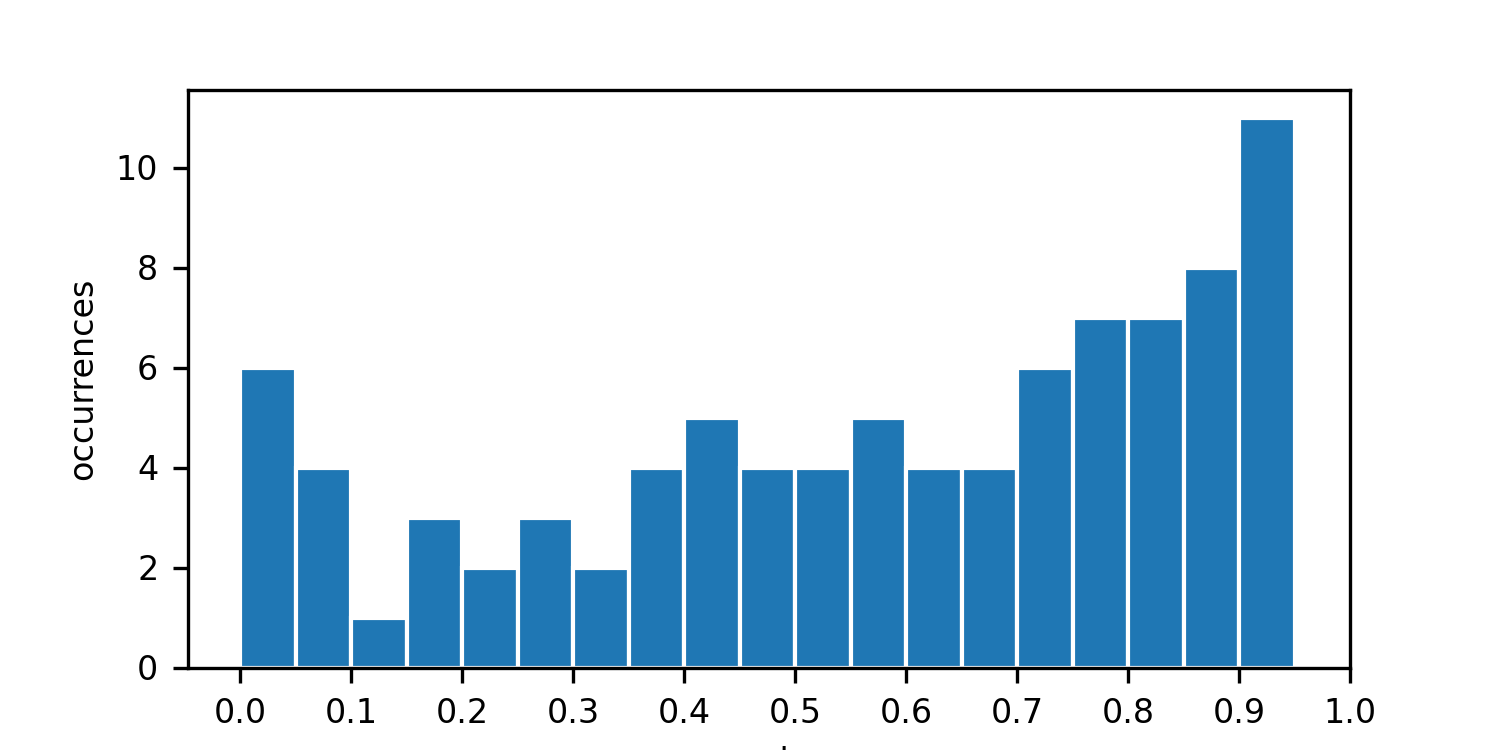
\includegraphics[width=5in]{6ffig1.png}
    \caption{10\% subset sample p-values}
    \label{6ffig1}
\end{figure}
\begin{mdframed}
    98 out of 100 samples confirm the null hypothesis while 2 out of 100 samples
    reject the null hypothesis.
\end{mdframed}
This is consistent with the full dataset's $p$-value of $p=0.97$ which indicates
a false positive rate of about $3\%$.

\end{document}